%\section{Simulation Study}

\subsection{Simulation Procedure}

To test algorithms (\ref{alg:EM-SO}) and (\ref{alg:P-EM-SO}), we ran a total of eight simulation experiments. For a given experiment, we simulated a total of $T \in \{10^3,10^5\}$ observations from an HMM with $N \in \{3,6\}$ hidden states and observations $y_t \in \bbR^d$, with $d \in \{3,6\}$. All possible combinations of $T$, $N$, and $d$ comprised a total of $2^3 = 8$ experiments. For each experiment, we simulated a total of five data sets. For every experiment and data set, $Y_t | X_t = i$ followed a normal distribution with mean $\mu^{(i)}$ and covariance matrix $\Sigma^{(i)}$, $\calN(\mu^{(i)},\Sigma^{(i)})$. We randomly defined $\mu^{(i)}$ and $\Sigma^{(i)}$ for every data set as follows:
%
\begin{equation}
    \mu^{(i)} \sim \calN(0,I), \quad \Sigma^{(i)} = \text{diag}(\exp(-2)), \qquad i \in \{1,\ldots,N\},
\end{equation}
%
where $I$ is the identity matrix.

We set the transition probability matrices of the generating process to depend upon both $T$ and $N$. The transition matrices depend upon $N$ because they must ($\Gamma \in \bbR^{N \times N}$), and they depend upon $T$ because we assume that the underlying Markov chain transitions a total of approximately 100 times. Intuitively, this simulates a observation sequences that are sampled at either low- or high- frequencies.

Denote the true transition probability matrix from an experiment with $T$ observations and $N$ hidden states as $\Gamma_{T,N}$. For our experiments, we set
%
\begin{gather*}
    \Gamma_{10^3,3} = 
    \begin{pmatrix} 
        0.9 & 0.05 & 0.05 \\
        0.05 & 0.9 & 0.05 \\
        0.05 & 0.05 & 0.9
    \end{pmatrix},
    \qquad
    \Gamma_{10^5,3} = 
    \begin{pmatrix} 
        0.999 & 0.005 & 0.005 \\
        0.005 & 0.999 & 0.005 \\
        0.005 & 0.005 & 0.999
    \end{pmatrix}
    \\
    \Gamma_{10^3,6} = 
    \begin{pmatrix} 
        0.9  & 0.02 & 0.02 & 0.02 & 0.02 & 0.02 \\
        0.02 & 0.9  & 0.02 & 0.02 & 0.02 & 0.02 \\
        0.02 & 0.02 & 0.9  & 0.02 & 0.02 & 0.02 \\
        0.02 & 0.02 & 0.02 & 0.9  & 0.02 & 0.02 \\
        0.02 & 0.02 & 0.02 & 0.02 & 0.9  & 0.02 \\
        0.02 & 0.02 & 0.02 & 0.02 & 0.02 & 0.9  \\
    \end{pmatrix},
    \\
    \Gamma_{10^5,6} = 
    \begin{pmatrix} 
        0.999  & 0.0002 & 0.0002 & 0.0002 & 0.0002 & 0.0002 \\
        0.0002 & 0.999  & 0.0002 & 0.0002 & 0.0002 & 0.0002 \\
        0.0002 & 0.0002 & 0.999  & 0.0002 & 0.0002 & 0.0002 \\
        0.0002 & 0.0002 & 0.0002 & 0.999  & 0.0002 & 0.0002 \\
        0.0002 & 0.0002 & 0.0002 & 0.0002 & 0.999  & 0.0002 \\
        0.0002 & 0.0002 & 0.0002 & 0.0002 & 0.0002 & 0.999  \\
    \end{pmatrix}.
\end{gather*}
%
We randomly defined the initial distribution as $\delta \sim \text{dir}(\onevec_N)$ for every experiment and data set.

\subsection{Optimization Procedure}

We estimated the parameters of the generating model for all five data sets and all eight experiments using six different inference algorithms. In particular, we used Algorithm (\ref{alg:EM-SO}) with $M=T$, Algorithm (\ref{alg:P-EM-SO}) with $M=T$, and Algorithm (\ref{alg:P-EM-SO}) with $M=10T$, each using either SVRG and SAGA within the M-step. Recall that Algorithm (\ref{alg:EM-SO}) uses the same E step of the Baum-Welch algorithm, but it incorporates stochastic optimization into the M step. Algorithm (\ref{alg:P-EM-SO}) occasional performs the E step from the traditional Baum-Welch algorithm, but it also incorporates a partial E step into its variance-reduced stochastic M step. The variable $M$ corresponds to the number of iterations of SAGA or SVRG that are performed at each M step of the algorithm, and $T$ is the length of the observation sequence. It is natural to set $M=T$ to approximately balance the computational load of the E step and the M step. However, since Algorithm (\ref{alg:P-EM-SO}) performs a partial E step in the middle of its M step, we set $M=10T$ for one experiment with Algorithm (\ref{alg:P-EM-SO}) to test if the partial E step within the M step was sufficient to perform inference.

We also estimated the HMM parameters using three baseline methods: BFGS \citep{Fletcher:2000}, Conjugate gradients \citep{Fletcher:1964}, and full-batch gradient descent.
%
All baselines were implemented using the Scipy library in Python \citep{Virtanen:2019}.

We sampled a total of five random parameter initializations for each data set and experiment, and ran all optimization algorithms for all parameter initializations corresponding to every data set / experiment pair. Each parameter initialization was re-used for each algorithm for consistency between optimization algorithms. Let $\bar y$ and $\bfQ$ denote the sample mean and sample covariance of the observation sequence $\{y_t\}_{t=1}^T$, respectively. Then, we initialized $\theta_0$ as
%
\begin{equation}
    \mu^{(i)}_0 \sim \calN(\bar y, \text{diag}(\bfQ)), \quad \Sigma^{(i)}_0 = \text{diag}(\bfQ), \qquad i \in \{1,\ldots,N\}.
\end{equation}
%
We initialized $\eta_0$ as
%
\begin{align*}
    \eta^{(i)}_0 &\sim \calN(0,1), & i & = 2,\ldots,N \\
    %
    \eta^{(i,j)}_0 &\sim \calN(-2,2^2), & i,j & = 1,\ldots,N, \qquad i \neq j.
\end{align*}
%
%If the 2-norm of the average estimated gradient $||\frac{1}{T}\sum_{t=1}^T \widehat \nabla F^{(k,m)}_t + \widehat \nabla G^{(k,m)}_t||$ ever fell below a tolerance of $10^{-8}$, we terminated the M-step of algorithm and moved on to the E-step. Likewise, if the relative change of the log-likelihood after one full E- and M- step of the EM algorithm ever fell below a tolerance of $10^{-10}$, we terminated the algorithm altogether. We found the ground truth MLEs by running the traditional EM algorithm until the relative change in the log-likelihood was on the order of machine precision $10^{-15}$.

Throughout the optimization procedure, we assume that $\Sigma^{(i)}$ is diagonal for all $i \in \{1,\ldots,N\}$, which is in line with the generating model described above. Further, because $\Sigma^{(i)}$ must have positive diagonal elements to be a valid covariance matrix, we parameterize $\Sigma^{(i)}$ as 
%
\begin{equation}
    \Sigma^{(i)} = 
    \begin{pmatrix}
        \exp(\rho_1)^2 & 0 & \ldots & 0 \\
        0 & \exp(\rho_2)^2 & \ldots & 0 \\
        \vdots & \vdots & \ddots & \vdots \\
        0 & 0 & \ldots & \exp(\rho_N)^2 \\
    \end{pmatrix},
\end{equation}
%
and perform inference on $\boldsymbol{\rho} = \begin{pmatrix} \rho_1, \rho_2, \ldots , \rho_N \end{pmatrix}$. Performing inference directly on $\boldsymbol{\rho}$ allows us to perform unconstrained optimization.

All six algorithms were initialized with step sizes of $\lambda_F = 1/3 \hat L_F$ and $\lambda_G = 1/3 \hat L_G$. The Lipschitz constants were initialized as $\hat L_F = \hat L_G = 100/3$ and updated during the optimization routine according to the procedure from section \ref{subsec:est_L}. 
%
All algorithms and baselines were run for a total of 12 hours on the Compute Canada Cedar cluster on nodes with 16GB of RAM.

\subsection{Simulation Results}


SVRG tends to converge faster than the baseline for all experiments, and SAGA tends to converge faster than the baselines for all experiments except for when $N=3$. The baselines are prone to converging to local minima, especially when $N=6$. Our method is still prone to converge to local minima, especially when $N=6$, but it performs better than BFGS for all experiments with the exception of $N = 3$ and $d = 3$, where BFGS achieves the highest log-likelihood after approximately 120 epochs. However, BFGS is a second-order method, so it is expected to outperform our first-order methods on a per-epoch basis when very close to the true solution.

Figure (\ref{fig:scatter_sim}) shows that many SVRG / SAGA experiments converge faster and to solutions with higher likelihood compared to BFGS. 
%
The data set displayed here is representative of the results from the other four data sets from each experiment. Nonetheless, we recreate Figure (\ref{fig:ll_trace_sim}) for the other four data sets of each experiment in the supplement. Analogous experiments for data sets with $T=10^3$ can also be found in the supplement. 

The algorithms which implement a partial E step appear to help the algorithm move to areas of high likelihood, especially within the first ~20 epochs of optimization. We show zoomed in versions of Figure (\ref{fig:ll_trace_sim}) in the appendix to highlight the advantages of the partial E step early in the optimization procedure.
%
\begin{figure}
    \centering
    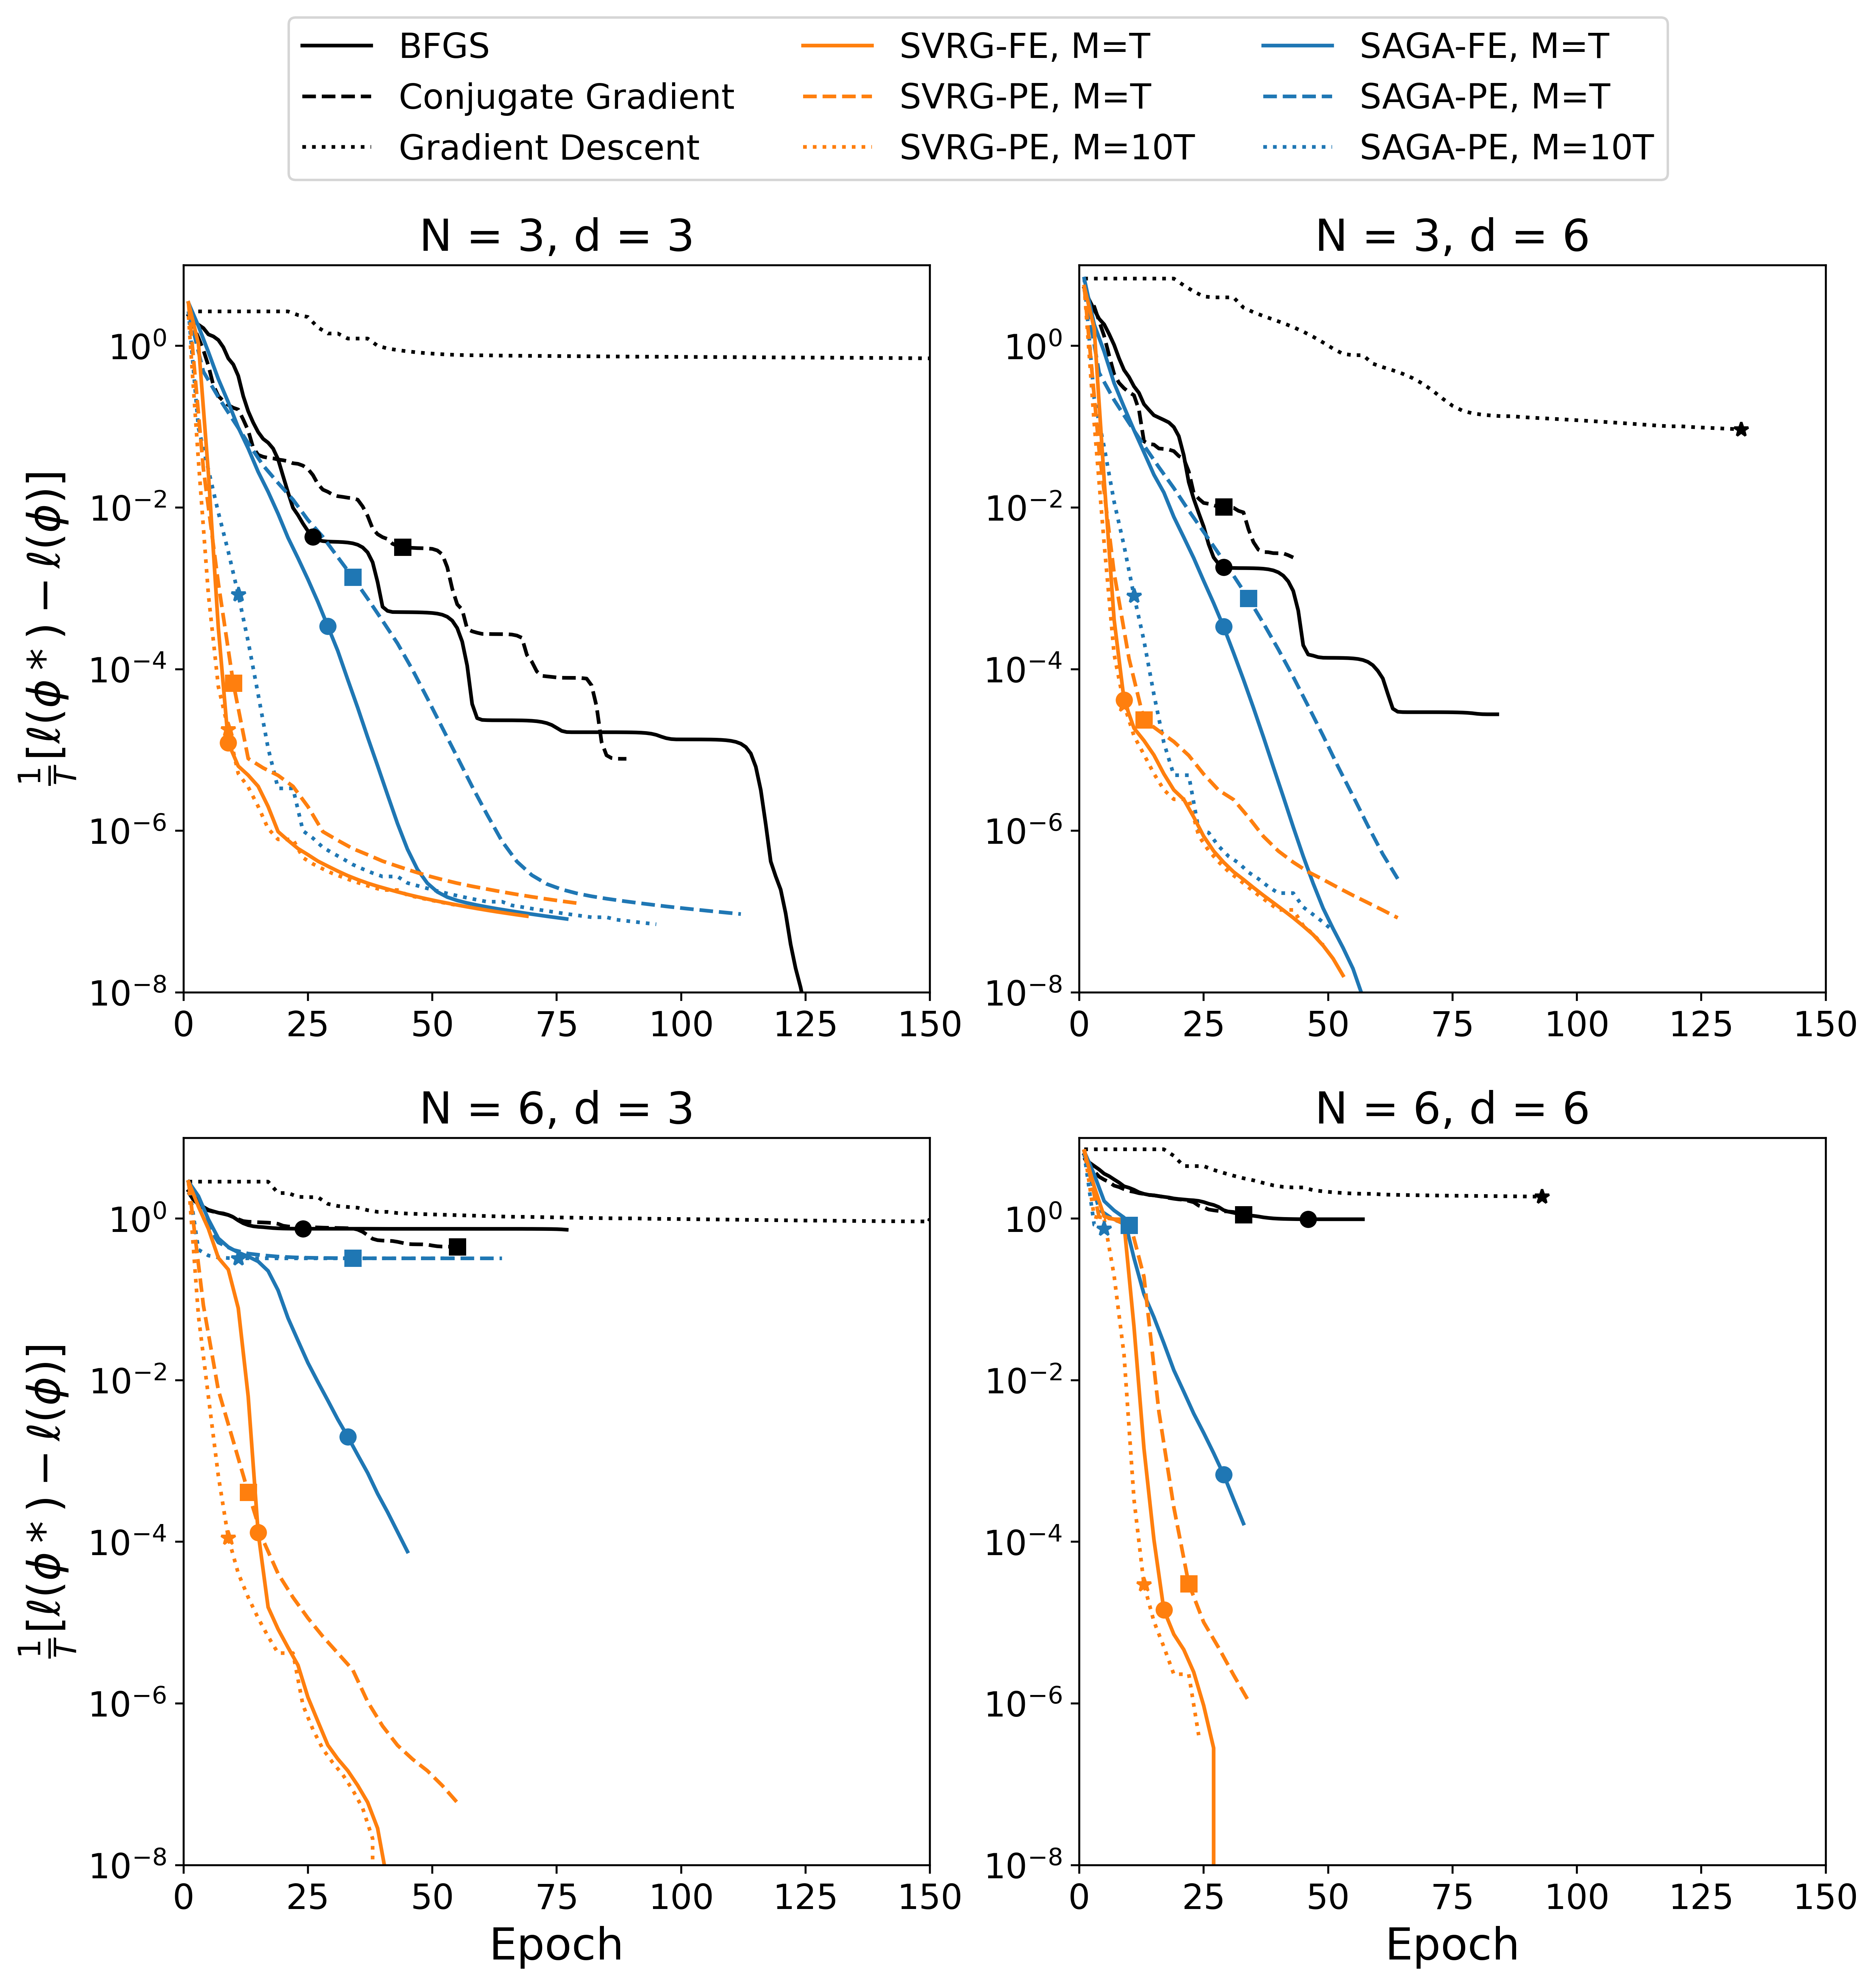
\includegraphics[width=6.5in]{../plt/log-like_v_epoch_T-100000-000.png}
    \caption{log-likelihood of the maximum log-likelihood minus the log-likelihood (all divided by $T$) at each epoch of a selected run of each optimization algorithm after 12 hours or 150 epochs (whichever came first) for the first data set of the experiment with $T=10^{5}$, $N=3$ and $d=3$ (top left), $N=3$ and $d=6$ (top right), $N=6$ and $d=3$ (bottom left), and $N=6$ and $d=6$ (bottom left). One epoch represents either one full E-step, $T$ iterations with the M-step, or one gradient step for full-gradient algorithms. The y-axis is on a log-scale. For each optimization algorithm, we display the random initialization that resulted in the highest likelihood after 12 hours. The dots on each figure correspond to the epoch and likelihood at convergence for each algorithm. Convergence is defined as the point at which the gradient norm of the log-likelihood (divided by $T$) was less than $10^{-2}$. We selected a tolerance of $10^{-2}$ because it was the lowest tolerance that all algorithms regularly converged to within 12 hours.}
    \label{fig:ll_trace_sim}
\end{figure}
%
\begin{figure}
    \centering
    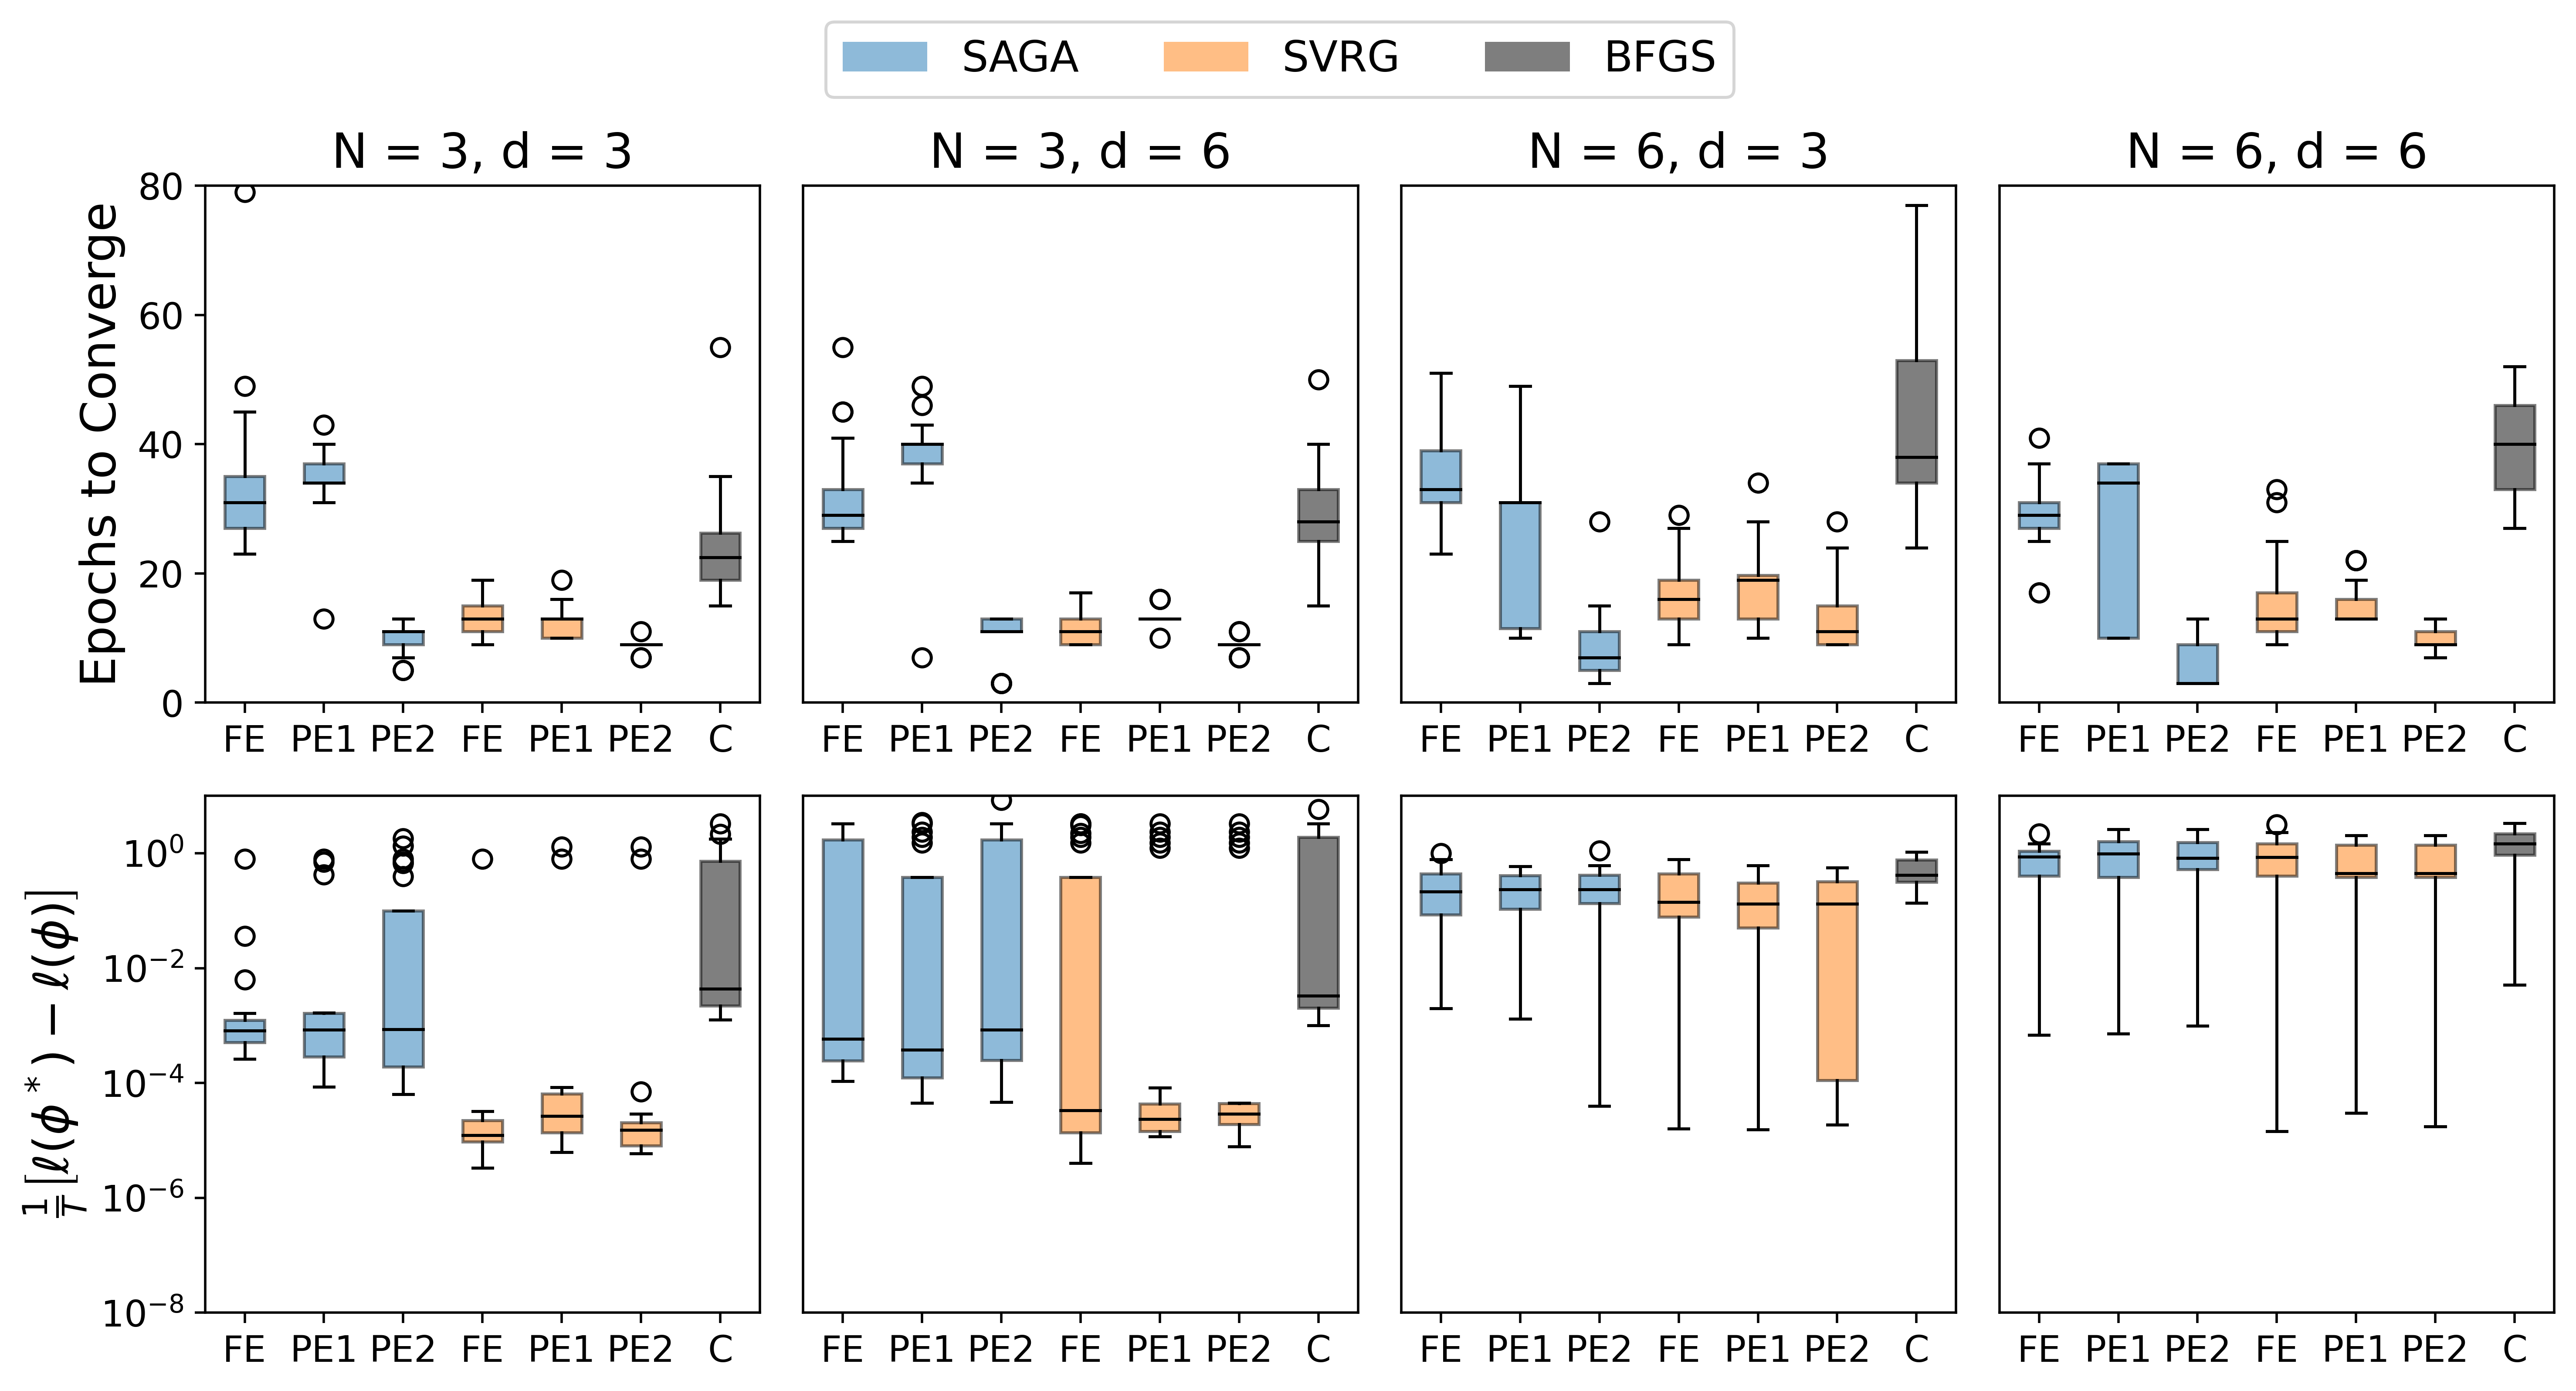
\includegraphics[width=6.5in]{../plt/boxplots_sim_T_100000.png}
    \caption{Box plots showing epochs to converge (top) and the log-likelihood of the maximum log-likelihood minus the log-likelihood (all divided by $T$) at convergence (bottom) for each optimization algorithm. NPE corresponds to Algorithm (\ref{alg:EM-SO}), PE1 corresponds to Algorithm (\ref{alg:P-EM-SO}) with $M=T$, and PE2 corresponds to Algorithm (\ref{alg:P-EM-SO}) with $M=10T$. Blue corresponds to SAGA and orange corresponds to SVRG. Results are shown for all simulation studies with $T=10^{5}$, $N=3$ and $d=3$ (left), $N=3$ and $d=6$ (left-middle), $N=6$ and $d=3$ (right-middle), and $N=6$ and $d=6$ (right). One epoch represents either one full E-step, $T$ iterations with the M-step, or one gradient step for full-gradient algorithms. The y-axis of the bottom row is on a log-scale.}
    \label{fig:boxplots_sim}
\end{figure}
%
\begin{figure}
    \centering
    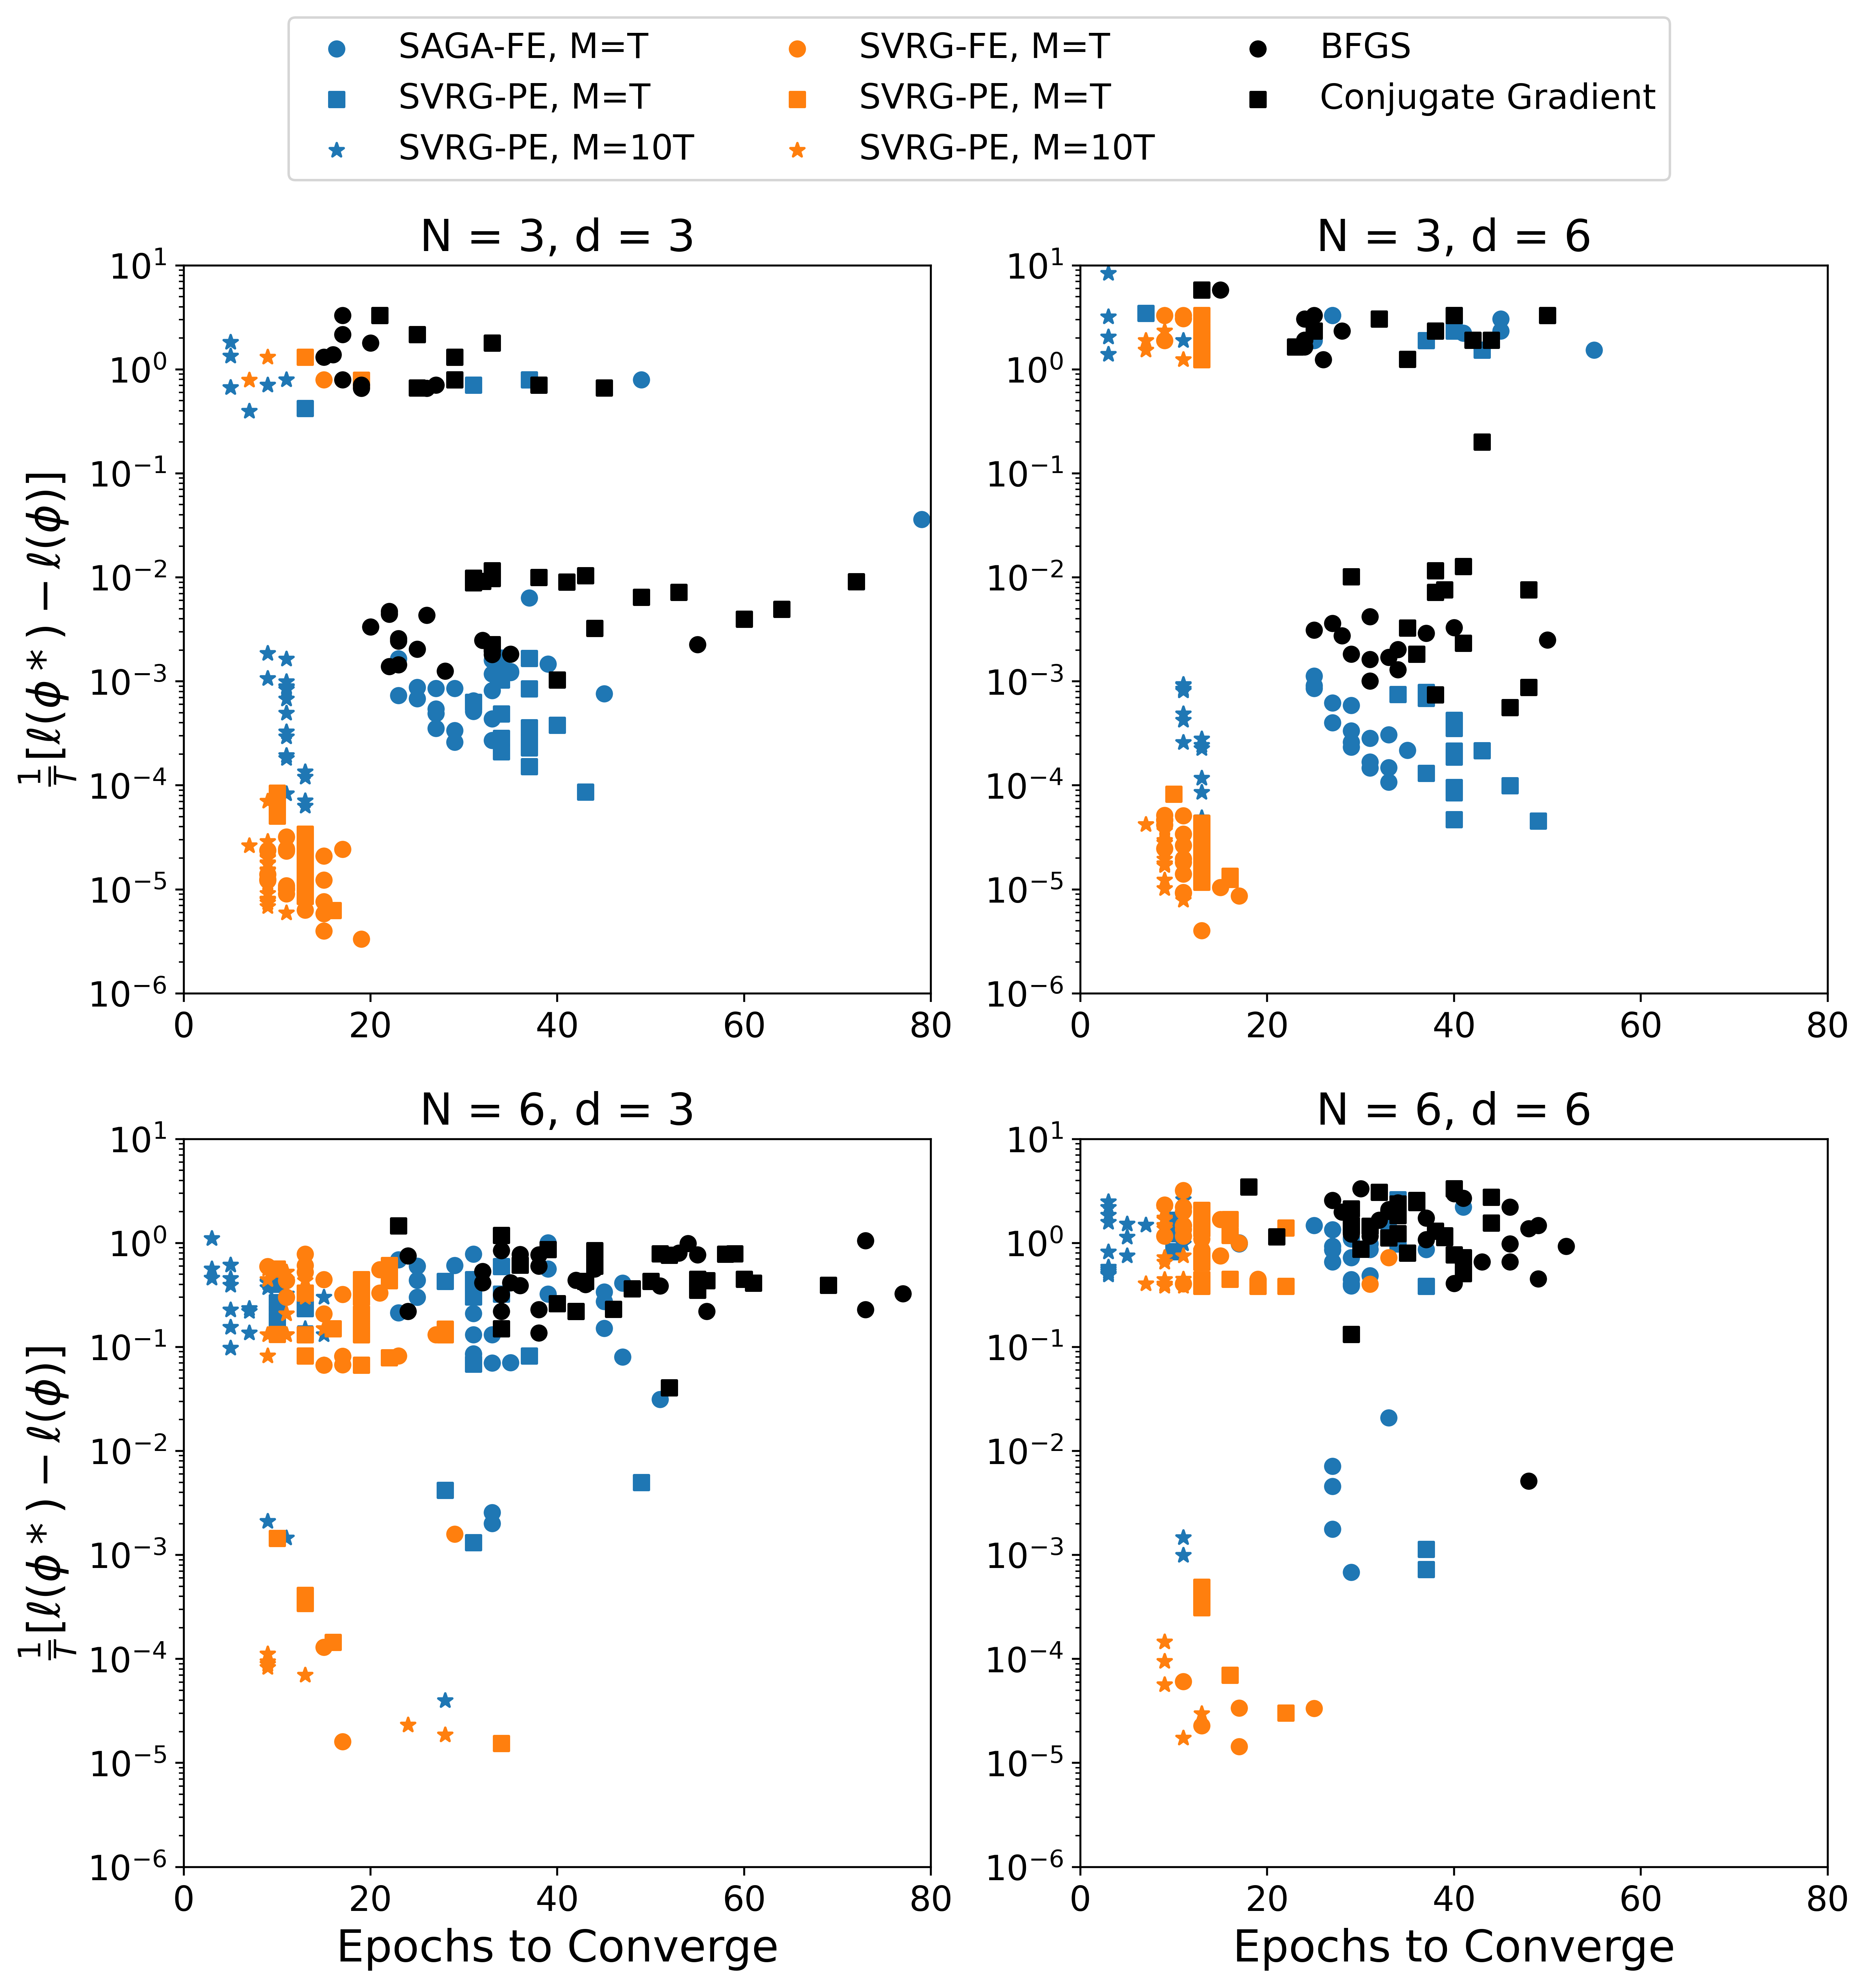
\includegraphics[width=6.5in]{../plt/scatter_sim_T_100000.png}
    \caption{Log-likelihood of the maximum log-likelihood minus the log-likelihood (all divided by $T$) at convergence versus epochs to converge for all simulation studies with $T=10^{5}$, $N=3$ and $d=3$ (top left), $N=3$ and $d=6$ (top right), $N=6$ and $d=3$ (bottom left), and $N=6$ and $d=6$ (bottom left). One epoch represents either one full E-step, $T$ iterations with the M-step, or one gradient step for full-gradient algorithms. The y-axis is on a log-scale.}
    \label{fig:scatter_sim}
\end{figure}
%
%Overall, SVRG appears to converge faster than SAGA for all algorithms. 
%This may be a function of our step size ($1/3 \hat L$), but that step size was selected based upon suggestions from the SAGA paper \citep{Defazio:2014}. 


%The partial E- step within Algorithm (3) looks to help primarily for experiments with $N=6$, especially for early epochs of the algorithm. This makes sense since the weights from the EM algorithm will be out of date quickly when the parameter estimates are poor early in the EM algorithm.

%SAGA without a partial E-step performs similarly to the EM algorithm in a per-epoch basis because SAGA is successfully converging for the M-step when $M = T$. However, it does not perform as well as the EM algorithm on a per-time basis because the M-step is significantly slower when using SAGA vs the closed-form solution. This behaviour is expected, and SAGA has a significant advantage over the EM algorithm in that it only requires gradients rather than sufficient statistics.

%mplementing a partial E-step shows that SAGA can outperform the EM algorithm when the parameter estimates are far from the optimal solutions and when the underlying HMM does not mix rapidly. This is likely because the weights of the $F$ and $G$ are very inaccurate at first, and updating them early in the optimization procedure yields a significant speed-up. In addition, if the Markov chain is rapidly mixing, then updates to $\gamma_{t_m}$ and $\xi_{t_m}$ at a single data point are more accurate. Future work may involve performing the partial-E step for many weights at once sequentially, depending upon the mixing time of the current estimate of $\eta_k$.